\section{SAT Model}
% This part is mandatory for groups of 4 students. Groups up to 3 students can choose between SAT and SMT, and will be given bonus points if they do both.

\subsection{Decision variables}
% Describe all the literals of your model and their semantics. For example, $\Delta_{i,j} = \text{true}$ iff the driver goes from city $i$ to city $j$.
Let $rb$ be the round robin tournament, $sts$ a schedule satisfying to the STS problem, and P, W, T the set of periods, weeks and teams respectively.
The satisfiability task is formalized by the following categories of propositions:
\begin{itemize}
    \item $matches\_schedule_{p, w, m} \leftrightarrow$ match $m$, denoting $rb_{m, w} = (t_1, t_2)$, takes place in period $p$ of week $w$
    \item $matches\_to\_periods_{t_1, t_2, p} \leftrightarrow$ $t_1$ plays against $t_2$ in period $p$
\end{itemize}
The optimization task, on the other hand, is expressed as follows.
\begin{itemize}
    \item $slots\_schedule_{p, w} \leftrightarrow$ team $sts_{p, w, 1} = t_1$ plays away
    \item $matches\_to\_slots_{t_1, t_2} \leftrightarrow$ $t_1$ plays away and $t_2$ plays at home
\end{itemize}

\subsection{Objective function}
Similarly to the other approaches, the objective is to minimize the absolute difference between the number of games played at home and away for each team.
Let $T$ be the set of teams and $A_t$ the number of times the team $t \in T$ plays away, the objective function translates into the following:
$$
k * = \underset{k \in \mathbb{N}}{\text{argmax}} \left( \forall t \in T, A_t \geq k \right)
$$
The chosen CP model allows to solve the optimization task independetly of the STS constraints using the $sts$ schedule computed in the satisfiability process. The optimization consists of a binary search of $k*$ in the interval $[1, \lfloor\frac{N-1}{2}\rfloor]$. Since SAT doesn't directly support optimization, a new set of optimizing constraints is introduced for every instance of $k$ .

The result is encoded in $slots\_schedule_{p, w}$, which cannot express the constraints alone, due to structural limitations of the encoding.
Instead \\$matches\_to\_slots_{t_1, t_2}$ is used: given a week $w$ and a period $p$, the team $sts_{p, w, 1} = t_1$ plays away if, and only if, the team $t_2 = sts_{p, w, 2}$ plays at home. Therefore, by definition:
$$
    \forall p \in P, w \in W.(slots\_schedule_{p, w} \leftrightarrow matches\_to\_slots_{sts_{p, w, 1}, sts_{p, w, 2}})
$$
Finally the optimization process is implemented by ensuring that for an instance $k \in [1, \lfloor\frac{N-1}{2}\rfloor]$:
$$
    \forall p \in P, t_1 \in T.(AtLeastK(matches\_to\_slots_{t_1, t_2} | t_2 \in T/\{t_1\}))
$$

\subsection{Constraints}
% Describe all the clauses of your model and their semantics. In particular, describe the encoding(s) that you used. Follow the indications given in Section 2.3 for main problem constraints, implied constraints, and symmetry breaking constraints.
\subsubsection{Every team plays once a week}
In a Round-Robin tournament $rb$, each team plays exactly once a week. 
Therefore the only problem is to ensure that for each week $w$, every match $rb_{m, w} = (t_i, t_j)$ is assigned to exactly one period $p$.

We enforce that every match is scheduled once:
$$
    \forall p \in P, w \in W.(ExactlyOne(matches\_schedule_{p, w, m} | m \in P))
$$
Finally no two matches are scheduled in the same period. 

We ensure that each match is scheduled to a unique period $p$ in the week $w$.
$$
    \forall m \in P, w \in W. ExactlyOne(matches\_schedule_{p, w, m} | p \in P)
$$
\subsubsection{Every team plays at most twice in the same period}
The constraint cannot be expressed using directly $matches\_schedule_{p, w, m}$, due to structural limitations of the encoding. 
Instead, we introduce the literal $matches\_to\_periods_{t_i, t_j, p}$: given a week $w$, the match $rb_{m,w}$ is scheduled in period $p$ if, and only if, the match $(rb_{m, w, 1}, rb_{m, w, 2}) = (t_1, t_2)$ takes place in period $p$. Therefore, by definition: 
$$
    \forall p \in P, w \in W, m \in P.matches\_schedule_{p, w, m} \leftrightarrow matches\_to\_periods_{rb_{m, w, 1}, rb_{m, w, 2}, p}
$$
Computationally this constraint soundly maps $matches\_schedule$ to \\$matches\_to\_periods$, which allow to express the main constraint:
$$
    \forall p \in P, t_1 \in T. AtMost2(matches\_to\_periods_{t_1, t_2, p} | t_2 \in T/\{t_1\})
$$
\subsection{Validation}
% See Section 2.4. The model \textbf{must} be implemented using at least Z3. Bonus points will be considered if a solver-independent language (e.g., Dimacs) is employed so as to play with different SAT solvers on the same model.
\subsubsection{Experimental design}
The model was written in Python by making use of the Z3 and the CVC5 library, which offers CaDiCaL and MiniSat as the underlying SAT solvers. The time elapsed to find an optimal solution, within the 300 second time limit, was measured and results presented in Fig.\ref{fig:SAT-result} . 
\subsubsection{Experimental results}
All solvers are able to find the optimal solution, which was much easier to find once the satisfying one was computed, but overall Z3 had the best performance in time and maximal size of the problem, i.e. $N=20$. On the other hand CaDiCaL was the worst, failing at $N=12$, while MiniSat stopped at $N=14$
\begin{figure}
    \centering
    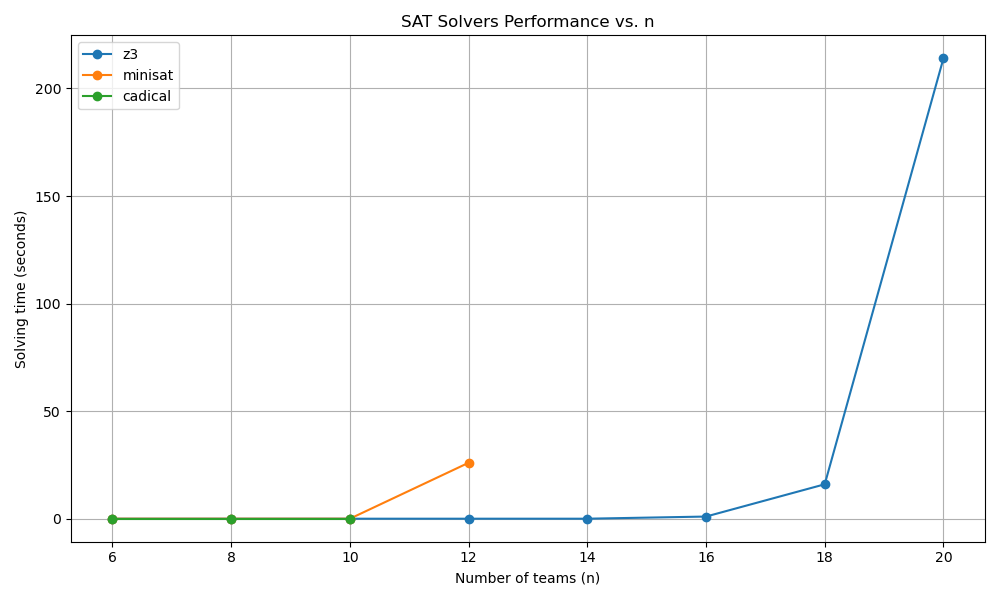
\includegraphics[width=0.8\linewidth]{img/SAT-result.png}
    \caption{SAT optimization}
    \label{fig:SAT-result}
\end{figure}